Décrire ce qui a été fait, ce qui est à faire, comment tout à été fait, ...

En gros, faire un état des lieux en utilisant la bibliographie.

\chapter{Introduction}%\markboth{Introduction}{}}
	\minitoc
	  \section{Historique}
Les premiers amas d'étoiles ont été catalogués par \textsc{Messier} en 1784, mais ils n'ont été identifiés comme tel qu'en 1814 par William \textsc{Herschel}. Étudiés depuis cette époque, notre connaissance
	observationnelle à leur propos n'a pas cessé de s'améliorer avec la progression des techniques d'observation.
	Le premier comptage d'étoiles complet fut effectué par \textsc{Bailey} en 1893. En 1905, \textsc{Plummer} et \textsc{von Zeipel}	ont utilisé les observations pour
	remonter à la distribution radiale des étoiles. \textsc{Von Zeipel} fit alors le rapprochement entre un amas et une sphère de gaz à l'équilibre isotherme.
	Parallèle encore utilisé aujourd'hui, bien qu'il soit contestable sur au moins un point : le libre parcours moyen d'une étoile est grand devant la taille du
	système, alors que pour une sphère de gaz c'est l'inverse.% ; le mouvement des étoiles et celui des particules d'un gaz sont eux-mêmes assez différent (~l'un consiste
	%en des orbites déterminé par le potentiel gravitationnel des étoiles alentour, l'autre n'est constitué que de ligne droite~).

\section{Définition d'un amas globulaire}
	Dans notre galaxie, un amas globulaire est, en général, décrit comme un très vieil amas d'étoiles, âgé d'environ 10 milliards d'années, que l'on trouve soit près du bulbe galactique,
	soit dans le halo. Mais l'âge absolu de ces objets est très difficile à mesurer.
%	Par ailleurs, pour les amas en dehors du groupe local, cette définition n'est plus suffisante :
%	amas globulaire et amas ouvert ont des âges proches les uns des autres
%	En effet, dés que l'on observe une galaxie un peu lointaine~\footnote{et même dans les nuages de Magellan}, les amas sont de plus en plus jeune~\footnote{dans les nuages de Magellan,
%	les âges varient entre $10^6$ et $10^9$ ans}.

%	Mais restons dans notre galaxie pour le moment : ne serait-ce que dans notre galaxie, les amas globulaire peuvent être très différent les uns des autres :
	Les amas de notre galaxie présentent des caractéristiques assez variées. Par exemple, l'amas le plus massif de notre galaxie --~$\omega$ Centauri~-- posséde une masse d'environ $5.10^6 M_\odot$
	tandis que celle du moins massif --~AM-4~--est d'environ $10^3 M_\odot$.
	Leur magnitude absolue~\footnote{De $M_V = -10.1$ pour $\omega$ Centauri à $M_V = -1.7$ pour AM-4} et distance au centre de la galaxie~\footnote{environ 20 kpc pour les plus proche du centre à 120 kpc pour AM-1} varie également dans de grandes proportions.
	Une partie des amas est concentrée autour du centre galactique tandis que d'autres évoluent dans le halo galactique.


	%%%% Temps caractéristiques
			Il est utile de décrire quelques temps caractéristiques de l'évolution de ces systèmes.
	\subsection{Temps dynamique}
		Le temps dynamique est le temps nécessaire à une particule pour traverser le système et donc se \og mettre au courant \fg~des changements ayant lieu.
		Il s'agit donc de la plus petite échelle de temps que nous puissions considérer pour l'évolution d'un système auto-gravitant.
		Pour l'obtenir, considérons un système de $N$ particules de même masse $m$, et de dispersion de vitesse $\sigma$. Les énergies potentielles et cinétiques du système
		peuvent être évaluées par :
		\begin{align}
			E_c = \frac{N}{2}m\sigma^2\qquad\mathrm{et}\qquad E_p = -\frac{G(Nm)^2}{R}
		\end{align}
		puis en supposant que le système à l'équilibre et en appliquant le théorème du \textsc{Viriel}~\footnote{Rappel : $2 E_c + U = 0$ avec $E_c$
		l'énergie cinétique et $U$ l'énergie potentielle}, nous obtenons :
		\begin{align}
			\sigma = \(\frac{GNm}{R}\)^{1/2}
		\end{align}
		Le temps dynamique est proportionnel au temps de croisement des particules du système. Ce dernier dépend du rayon de l'objet
		considéré et de la vitesse caractéristique des étoiles dans le système, ou encore, de la dispersion de vitesse du système :
		\begin{align}
			T_{cr} \propto T_d = \frac{R}{\sigma} \label{Td:sig}
		\end{align}
		En injectant notre expression pour la dispersion de vitesse, nous avons le temps dynamique :
		\begin{align}
			T_d = R\(\frac{R}{GNm}\)^{1/2} = \sqrt{\frac{R^3}{GM}} \propto \frac{1}{\sqrt{G\rho}}
			\label{Td:rho}
		\end{align}
		avec $M = Nm$ la masse totale du système.
	\subsection[Temps de relaxation]{Temps de collision ou temps de relaxation à 2 corps}
		Le temps de collision est par définition le temps mis par les interactions à 2 corps pour modifier d'un ordre de grandeur la vitesse des particules du système.
		Le détail pour le calcul de ce temps peut-être trouvé dans~\cite{ThNico} et~\cite{CoursJP}. Il s'écrit, en fonction du temps de croisement :
		\begin{align}
			T_{c} = \frac{3N}{8\ln\(\frac{3N}{4\pi}\)}T_{cr}
		\end{align}

		Ce temps est donc proportionnel au temps dynamique $T_d$ par l'intermédiaire du temps de croisement.



	%%%% Vlasov-Poisson
		\section{Syst\`{e}me de \textsc{Vlasov}-\textsc{Poisson}}

	Nous allons \'{e}tudier ici des syst\`{e}mes de $N$ particules en interaction gravitationnelle dans la limite $N$ tend vers l'infini.
	Dans une approche formelle, \'{e}crire les \'{e}quations de \textsc{Newton} parait illusoire dans ce contexte, il convient d'utiliser le formalisme de la physique statistique et de d\'{e}crire le syst\`{e}me par une fonction de distribution not\'{e}e $f$.
	Cette derni\`{e}re permet de calculer la probabilit\'{e} pour une particule test de masse $m$ d'\^{e}tre dans un voisinage de la
	position $\left[\vec{r},\vec{p}\right]^\top$ dans l'espace des phases ; elle
	s'exprime en nombre par unit\'{e} de volume par impulsion au cube : $\left[ f\right] = m^{-3}p^{-3}$.

	La conservation du nombre de particules, les \'{e}quations d'\textsc{Hamilton}, et les hypoth\`{e}ses classiques d'ind\'{e}pendance et d'indiscernabilit\'{e} (voir ~\cite{CoursJP}~)) permettent d'obtenir l'\'{e}quation de \textsc{Boltzmann} :
	\begin{align}
		\frac{\partial f}{\partial t} +\frac{\vec{p}}{m}\frac{\partial f}{\partial \vec{r}} - m\frac{\partial f}{\partial \vec{p}} \frac{\partial \psi}{\partial \vec{r}} = N^2 G C(\vec{r},\vec{p} t)
		\label{Fok-Plan}
	\end{align}
	o\`{u} la fonction
	\begin{align}
		\psi(\vec{r},t)=-Gm\int\frac{f(\vec{r}\,^{\prime},\vec{p}\,^{\prime}, t)}
		{\left|\vec{r}-\vec{r}\,^{\prime}\right|}
		d^3\vec{r}\,^{\prime}d^3\vec{p}\,^{\prime}
		\label{pot-grav}
	\end{align}
	est appel\'{e}e potentiel de champ moyen du syst\`{e}me.
	
	Nous reviendrons plus loin sur les hypoth\`{e}ses statistiques permettant d'obtenir cette \'{e}quation car il s'av\`{e}re que certaines sont discutables dans le contexte gravitationnel et vraisemblablement \`{a} l'origine ce certains probl\`{e}mes. Tant que nous pouvons consid\'{e}rer que les  interaction \`{a} deux corps (collisions) n'affectent pas la dynamique du syst\`{e}me, hypoth\`{e}se qui sera discut\'{e}e plus tard, le
	terme  $ C(\vec{r},\vec{p}, t) $ est n\'{e}gligeable. Nous obtenons alors l'\'{e}quation de
	\textsc{Vlasov-Poisson} ou \textsc{Boltzmann} sans collision :
	\begin{align}
		\frac{\partial f}{\partial t} +\frac{\vec{p}}{m}\frac{\partial f}{\partial \vec{r}} - m\frac{\partial f}{\partial \vec{p}} \frac{\partial \psi}{\partial \vec{r}} = 0
		\label{Vla-Pois}
	\end{align}

	Tout les \'{e}tats stationnaires des syst\`{e}mes que nous \'{e}tudierons par la suite seront solution de cette \'{e}quation.
	L'une des grandeurs physique fondamentale qui motivera notre int\'{e}r\^{e}t tout le long de notre travail est la densit\'{e} volumique de masse $-$ que nous appellerons souvent densit\'{e} $-$ s'\'{e}crit simplement comme une loi marginale de $f$ :
	\begin{align}
		\rho(\vec{r},t) = m\int f(\vec{r},\vec{p},t) d\vec{p} \label{def-dens}
	\end{align}

\chapter{Propriétés générales des systèmes auto-gravitants}

J'ai mis ce chapitre dans l'intro, il permet de décrire ce que l'on sait des amas globulaires. Il faut éviter toute référence précise au modèle de King. L'idée est de montrer l'évolution de la pente avec l'âge, et les deux catégories d'amas avec ou sans c\oe ur.
 Il faudrait rajouter une section sur les galaxies, voire les amas de galaxies en utilisant l'article de revue de Merritt.

	\minitoc
	\section{Introduction}
			Nous avons dénombré environ 150 amas globulaires dans notre galaxie. Sur ces amas, $20\%$ ont un cœur effondré. %, mais pas les $80\%$ restants.
	Depuis une centaine d'année, des astrophysiciens --~tel \textsc{Chandrasekhar}, \textsc{King}, ...~--
	tentent d'expliquer à l'aide de différents modèles les propriétés observées de ces objets.
	Nous avons étudié dans les chapitres précédents deux \og grands modèles \fg~décrivant ces états d'équilibres,
	mais le point qui intéresse plus spécialement les physiciens est l'évolution des amas : comment en sont-ils
	arrivés là et que pourraient-ils devenir ?

	Du fait de nos développements théoriques dans les chapitres précédents, nous avons la possibilité de lier
	$W_0$ à la pente de la densité d'un modéle de \textsc{King},  modèle le plus utilisé lorsqu'il s'agit d'ajuster des données.
%	Dans~\cite{King-1966AJ}, Ivan R. \textsc{King} donne quelques explications sur pourquoi le modéle de la sphère isotherme singuliére
%	n'est pas utilisé et l'intérêt d'utiliser des modéles limité spatialement.

	Sur les graphes~\ref{effondre} et~\ref{pas_effondre} nous pouvons voir la courbe de densité
	d'un amas, respectivement, au cœur effondré et au cœur ne l'étant.
%	Le scénario utilisé ici, et qui sera étudié plus en détaille lors des simulations numériques, consiste en un \og~effeuillage~\fg progressif de l'amas : sa présence
%	dans le potentiel galactique lui fait perdre, petit à petit, des étoiles. Cette perte d'étoile va faire rétrécir le cœur de l'amas selon le processus mentionné dans
%	la section~\ref{petit_scenar} (~dû à la capacité calorifique négative~).
%	Une perte d'étoile trop importante entraînant ainsi un effondrement.
%	Le scénario ainsi évoqué peut-être résumé, de façon schématique, comme sur le schéma~\ref{schema-effondrement}.
%	Les études développées dans les chapitres précédents nous amènent à considérer que le système se comporte comme ayant un cœur et un halo bien distinct, l'un
%	caractérisé par sa densité constante, l'autre par la pente avec laquelle décroit la dite densité.
	Les études précédentes nous permettent de considérer que les objets étudiés possèdent une structure cœur-halo. Le cœur est la région dans laquelle la densité est constante ; le halo est la région dans laquelle la densité
	décroit selon une loi en $r^{-\alpha}$, la constante $\alpha$ étant appelée la pente du halo.

	\begin{figure}[ht!]
		\begin{minipage}[b]{0.48\linewidth}
			\begin{center}
%				\begin{gnuplot}[terminal=pdf,scale=0.50]
%					set xlabel "Distance au centre"
%					set ylabel "Densitee adimensionee et normalisee"
%					set title "Profil de densite de NGC 1904"
%					plot 'NGC1904.res' u 1:2 w p title "Densite de NGC 1904", '' u 1:2 smooth bezier not
%				\end{gnuplot}
%					plot '../Amas/res/NGC1904.res' u 1:2 w p title "Densite de NGC 1904", '' u 1:2 smooth bezier not
%				\includegraphics[scale=0.7]{graphe/NGC1904-2.pdf}
				\includegraphics[width=1.0\linewidth]{graphe/NGC1904-2.pdf}
				\caption{\footnotesize{Profil non effondré : \mbox{NGC 1904}} \label{pas_effondre}}
%				\begin{figure}[h]
%					\includegraphics[scale=0.5]{graphe/NGC1904.pdf}
%					\caption{Profil non effondré : NGC 1904 \label{effondre}}
%				\end{figure}
			\end{center}
		\end{minipage}\hfill
		\begin{minipage}[b]{0.48\linewidth}
			\begin{center}
%				\begin{gnuplot}[terminal=pdf,scale=0.50]
%					set xlabel "Distance au centre"
%					set ylabel "Densitee adimensionee et normalisee"
%					set title "Profil de densite de Terzan 2"
%					plot 'Terzan_2.res' u 1:(($2>2)?0:$2) w p title "Densite de Terzan 2", '' u 1:2 smooth bezier not
%				\end{gnuplot}
%					plot '../Amas/res/Terzan_2.res' u 1:(($2>2)?0:$2) w p title "Densite de Terzan 2", '' u 1:2 smooth bezier not
%				\includegraphics[scale=0.7]{graphe/Terzan_2.pdf}
				\includegraphics[width=1.0\linewidth]{graphe/Terzan_2.pdf}
				\caption{\footnotesize{Profil effondré : \mbox{Terzan 2}} \label{effondre}}
%				\begin{figure}[h]
%					\includegraphics[scale=0.5]{graphe/NGC1904.pdf}
%					\caption{Profil effondré : NGC 5946 \label{pas_effondre}}
%				\end{figure}
			\end{center}
		\end{minipage}
%		\caption{Exemple de profil de densité}
	\end{figure}
\normalsize


	\section[Lien]{Lien entre données et paramètres\label{amas}}
		\subsection{Préliminaire}
%	Ce qui va nous intéresser ici, c'est de pouvoir lier à chaque étape d'évolution d'un amas, et donc à son âge,
%	une pente.
	Notre objectif est de trouver une relation entre l'âge d'un amas et la pente de son halo.
	%Nous avons donc besoin d'une relation entre cette quantité et l'âge de l'amas, si une telle relation existe.
	Nous avons alors utilisé le temps de relaxation donné dans le catalogue de \textsc{Harris}~\cite{Harris}.
	Pour obtenir les pentes des amas, nous avons utilisé les relevés observationnels~\cite{Trager-graphe}. % (~les données ainsi obtenues et utilisées sont dans la table~\ref{pente-Tc:BSP}~).
	Nous avons commencé par calculer les pentes directement sur les courbes avec un double décimètre, n'ayant alors pas pu obtenir les données correspondant aux graphiques.
	Après avoir tracé la pente mesurée en fonction du temps de relaxation à 2 corps, nous avons ajusté la
	courbe ainsi obtenue par une droite d'équation $ \alpha = \mathrm{pente} = a \log_{10}(T_c) + b$ (~graphe~\ref{Pente-lin}~).
	\begin{figure}[hbt!]
		\centering \includegraphics[scale=0.9]{graphe/Pente-Tc.pdf}
		\caption{Évolution des pentes pour différents âges}
		\label{Pente-lin}
	\end{figure}
%	\begin{table}[hbt!]
%		\begin{center}
%			\begin{tabular}{|c|c|c|}
%				\hline
%				Coefficient & Valeur & Erreur \\
%				\hline
%				\hline
%				$a$       &        $-1.19506$   &   $\pm 0.1576$ (~$13.19\%$~) \\
%				\hline
%				$b$       &        $2.52082$     &   $\pm 1.213$   (~$48.11\%$~) \\
%				\hline
%			\end{tabular}
%		\end{center}
%		\caption{Valeur des coefficients donnée par l'ajustement pour les pentes}
%		\label{pente-lin-coeff}
%	\end{table}

	Cette approche indiquant clairement une relation linéaire entre ces deux paramètres, nous avons décidé d'entreprendre une démarche plus globale et automatique.
	Pour commencer, nous avons donc récupéré les données auprès des auteurs de l'article sur~\cite{TragerTable}. Nous nous sommes alors confronté au problème des unités.

\subsection{Retraitement}
	Le graphique~\ref{Pente-lin} a été obtenu en utilisant~\cite{Trager-graphe} avec ses unités. % (~les données permettant de retracer, nous les avons finalement trouvé,
%	les graphiques de cet article sont données dans~\cite{TragerTable}~).
	La pente donnée ici n'est donc pas la pente de la densité, mais de la brillance de surface de l'objet en fonction d'un rayon en seconde d'arc.
	Le premier traitement à effectuer consiste donc à transformer cette brillance de surface par arc seconde carrée en une densité (~kilogramme par kilomètre au cube~).

	Une définition de cette brillance de surface, telle qu'elle semble avoir été utilisée, peut-être trouvé dans~\cite{SBP}.
	Comme indiqué dans ce texte, la brillance de surface va s'écrire :
	\begin{align}
		\mu_V = \mu_{\mathrm{ref}} - 2.5 \log_{10}\(\frac{f/\Omega}{f_{\mathrm{ref}}/\Omega_{\mathrm{ref}}}\)
		\label{mu_V}
	\end{align}
	avec $\Omega$ l'angle solide, exprimé en seconde d'arc au carrée, sous lequel nous voyons l'objet.
%	\begin{align}
%		\mu_V = m_V - 2.5 \log_{10}\(\frac{(1\mathrm{"})^2}{\Omega}\)
%		\label{mu-astuce}
%	\end{align}
%	avec $m_V$ la magnitude apparente de l'objet sur une seconde d'arc au carrée.

	Cette définition rappelle celle de~\cite{Trager-graphe}, section~3.2.3 :
	\begin{align}
		\mu = -2.5 \log\(\frac{10^{-0.4 m_2} - 10^{-0.4 m_1}}{\pi \(r_2^2 - r_1^2\)}\)
		\label{Trager-eq}
	\end{align}
%	où ils prendraient comme référence les points autour de celui considéré (~ou quelque chose comme ça~),
	$m_i$ étant la magnitude en un point de l'objet et $r_i$ le rayon en seconde d'arc pour ce point.
	Par conséquent, les unités de $\mu$ sont un flux par arc seconde carrée en échelle logarithmique :
	\begin{enumerate}
		\item $10^{-0.4 m_i}$ est proportionnel à un flux, % (~ou au rapport d'un flux par rapport à un flux de référence !?!~),
		\item $r_i$ est le rayon de l'objet au point $i$ en seconde d'arc,
		\item[$\Rightarrow$] nous avons donc bien notre flux par seconde d'arc au carrée.
	\end{enumerate}
	Pour pouvoir revenir aux quantités que nous cherchons, il va falloir calculer un peu :
	\begin{align}
		\mu = -2.5 \log\(\frac{10^{-0.4 m_2} - 10^{-0.4 m_1}}{\pi \(r_2^2 - r_1^2\)}\) &\equiv -2.5 \log\(\frac{F}{\pi \(r_2^2 - r_1^2\)}\) \text{avec $F$ le flux}\notag \\
		\intertext{par rapport à toute la documentation que j'ai trouvé, le $\log$ correspond ici à $\log_{10}$ et non à $\ln$.}
		\Rightarrow \frac{F}{\pi \(r_2^2 - r_1^2\)} &= 10^{-\mu/2.5} \label{F--mu} \\
		\intertext{Grâce à~\cite{McL}, nous avons les rapports masse luminosité :}
		\Upsilon &= \frac{M}{L} \label{M/L}\\
		\intertext{or}
		F &= \frac{L}{4\pi D^2} \label{def-F}\\
		\intertext{avec $D$ la distance soleil--amas. D'où}
		\frac{L}{4 \pi^2 \(r_2^2 - r_1^2\) D^2} &= \frac{M}{4 \pi^2 \Upsilon \(r_2^2 - r_1^2\) D^2} = 10^{-\mu/2.5} \notag \\
		\intertext{en combinant~\ref{F--mu}, \ref{M/L} et~\ref{def-F}.}
		\Rightarrow \frac{M}{4\pi \(r_2^2 - r_1^2\)} &= \pi\Upsilon D^2 10^{-\mu/2.5} \notag \\
		\intertext{Mais $r_2^2 - r_1^2 \propto r_i^2$ doit être converti en mètre :}
		%r_2^2 - r_1^2 &\propto r_i^2 \Rightarrow \(D \tan(r_i)\)^2 \varpropto \(D r_i\)^2 \notag \\
		\Rightarrow \frac{M}{4\pi \(D \tan(r_i/3600)\)^2} &= \pi\Upsilon D^2 10^{-\mu/2.5} \label{M-don}
	\end{align}
	Normalement, nous avons maintenant une masse surfacique donnée par~\ref{M-don}.
%	mais, étonnamment, la conversion de seconde d'arc à mètre n'a fait paraître
%	aucun facteur numérique !!! J'ai peut-être un peu trop truandé.

	Les rapports masse-luminosité peuvent être trouvés dans~\cite{McL}, mais cette article ne contient que 40 des 140 amas de notre galaxie.
%	mais il n'y a qu'une quarantaine de rapport comparé à notre échantillon d'environ 140 amas.
	Par contre, il est aisé de remarquer que ces rapports sont
	en moyenne très peu différents de la valeur $\Upsilon = 2$ avec une valeur minimum de $1.87$ pour NGC 4147 et une valeur maximum de
	$2.66$ pour NGC 6441. Dans la suite, nous prendrons donc $\Upsilon = 2$.
%	Nous avons alors utilisé les données du catalogue pour redimensionner le tout, mais pour passer à la densité, nous avons besoin du rapport masse
%	sur luminosité de l'amas qui peut-être trouvé dans~\cite{McL}.
%	Cet article ne donne qu'une quarantaine d'amas sur les 150 de notre galaxie, mais les valeurs de ces rapports étant compris entre $1.87$ pour NGC 4147
%	(~et quelques autres~) et $2.66$ pour NGC 6441, et tournant surtout autour de $2$, nous pouvons supposer que ces rapports sont les mêmes pour chaque amas et
%	valent $\Upsilon = \frac{M}{L} = 2$.
%	Selon~\cite{Trager-graphe}, nous avons donc :
%	\begin{align}
%		\mu_V &\propto \text{Flux par $m^{-2}$} = \frac{L}{4\pi D^2} \\
%		\intertext{or}
%		L &= \frac{M}{\Upsilon} \notag \\
%		\intertext{donc}
%		\mu_V &= \frac{M}{4\pi D^2 \Upsilon} \notag \\
%		M &= \Upsilon \mu_V 4\pi D^2
%	\end{align}
%	avec $D$ la distance entre nous et l'amas. Nous pouvons supposer que cette distance est la même quelque soit l'étoile considéré dans l'amas
%	(~$D_{min} = 3000\mathrm{pc} \gg R_{amas} \approx 10\mathrm{pc}$~).

%	Du fait des rapports masse-luminosité manquant, notre échantillon d'une quarantaine d'amas est passé à seulement 12 amas.

\subsection{Résultat}
	Le calcul de pente a été refait en utilisant : les données de l'article~\cite{TragerTable}, le traitement décrit ci-dessus, et le critère donné dans la section~\ref{pente-critére}.
	Nous obtenons alors le graphique~\ref{Pente-lin_dim}, l'ajustement utilisant la fonction
	$f(T_c) = a \log(T_c) + b$ (~les coefficients ont été donnés dans la table~\ref{pente-lin-coeff_dim}~).
	Nous avons donc maintenant une relation linéaire entre l'âge de l'amas et la pente du halo.

	\begin{figure}[hbt!]
%		\centering \includegraphics[scale=0.9]{../Amas/Graphe_Rapport/pente-Tc.pdf}
		\centering \includegraphics[scale=0.9]{graphe/pente-Tc.pdf}
		\caption{Évolution des pentes pour différents âges}
		\label{Pente-lin_dim}
	\end{figure}
	\begin{table}[hbt!]
		\begin{center}
			\begin{tabular}{|c|c|}%c|}
				\hline
				Coefficient & Valeur \\ %& Erreur \\
				\hline
				\hline
				$a$       &         $-2.3341$   \\ %&    $\pm 0.2075$      (~$32.34\%$~) \\
				\hline
				$b$       &         $16.913$   \\  %&    $\pm 1.638$       (~$199.5\%$~) \\
				\hline
			\end{tabular}
		\end{center}
		\caption{Valeurs des coefficients donnée par l'ajustement pour les pentes pour le temps de croisement}
		\label{pente-lin-coeff_dim}
	\end{table}

	Nous avons également utilisé le catalogue de \textsc{Harris} pour obtenir le lien entre la pente du halo et le temps dynamique
	grâce à l'équation~\ref{Td:sig}. Nous obtenons alors le graphique~\ref{Pente-Td-lin}.
	\begin{figure}[hbt!]
%		\centering \includegraphics[scale=0.9]{../Amas/Graphe_Rapport/pente-Td.pdf}
		\centering \includegraphics[scale=0.9]{graphe/pente-Td.pdf}
		\caption{Évolution des pentes pour différents âges dynamiques}
		\label{Pente-Td-lin}
	\end{figure}
	\begin{table}[hbt!]
		\begin{center}
			\begin{tabular}{|c|c|}%c|}
				\hline
				Coefficient & Valeur \\ %& Erreur \\
				\hline
				\hline
				$a$       &        $-1.6567$   \\ %&   $\pm 0.6523$      (~$278.9\%$~) \\
				\hline
				$b$       &        $1.8927$     \\ %&   $\pm 2.825$       (~$88.57\%$~) \\
				\hline
			\end{tabular}
		\end{center}
		\caption{Valeurs des coefficients donnée par l'ajustement pour les pentes pour le temps dynamique}
		\label{pente-Td-lin-coeff}
	\end{table}

	Sur la figure~\ref{Pente-lin_dim}, nous pouvons noter la présence de 2 points avec des pentes inférieures à $-10$. Ces points correspondent aux amas NGC 5024 et NGC 5139
	(~leurs densités sont donnée en annexe, page~\pageref{Graphe-bofbof}~) pour lesquelles la détermination des pentes n'a pas été très concluante.
	\FloatBarrier



	\section{Interprétation}
		Nous avons maintenant une équation liant la valeur de la pente au temps de relaxation : $ \mathrm{pente} = \alpha = d * \log_{10}(T_c) + e $ (~coefficients table~\ref{pente-lin-coeff_dim}~)
et une autre liant la pente à $W_0$ : $ \alpha = a e^{ b W_0 } + c $.
En combinant ces deux équations, nous pouvons obtenir une relation entre le temps de
relaxation et $W_0$ :
\begin{align}
	\mathrm{pente} &= d \log_{10}(T_c) + e = a e^{b W_0} + c \notag \\
	\Rightarrow W_0 &= \frac{1}{b} \ln\( \frac{d \log_{10}(T_c) + e - c}{a} \) \label{Tc:W0->fct}
\end{align}
avec :
\begin{table}[h!]
	\begin{center}
		\begin{tabular}{|c|r|}
			\hline
			Coefficient	&	Valeur \\
			\hline
			\hline
			$a$		&	$ -10.0698 $ \\
				\hline
			$b$		&	$ 0.220152 $ \\
			\hline
			$c$		&	$ -1.53409 $ \\
			\hline
			$d$		&	$ -2.3341 $ \\
			\hline
			$e$		&	$ 16.913 $ \\
			\hline
		\end{tabular}
	\end{center}
\end{table}

Le comportement que nous avions observé en étudiant le modèle de \textsc{King}, à savoir une évolution de la pente avec $W_0$, se retrouve avec l'âge de notre amas. Ce qui nous a permis de relier
l'âge et $W_0$.
Il nous reste à interpreter ces résultats, ce que nous allons faire dans la section suivante.


	\section{Petit Scénario\label{petit_scenar}}
		%Nous avons vu que les courbes~\ref{King_Modele-test} peuvent être divisées en deux parties : l'une, caractérisée par une densité constante, constituant un cœur, et l'autre constituant un halo.
%Nous allons donc considérer un amas d'étoile composé d'un cœur dense et d'un halo.
%Le halo a peu de gravité et se comporte comme un gaz parfait.
%Le comportement observé dans notre étude est résumé sur le schéma~\ref{schema-effondrement} :
%
	\begin{figure}[ht!]
		\begin{minipage}[b]{0.20\linewidth}
			\begin{center}
				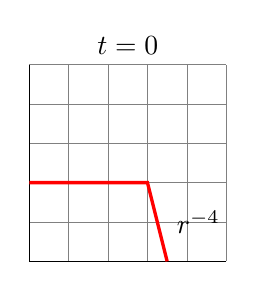
\begin{tikzpicture}
%					Tracé de la grille :
					\draw[step=.5cm,gray,very thin] (0,0) grid (2.5,2.5);
%					Tracé des axes :
					\draw (0,0) -- (0,2.5);
					\draw (0,0) -- (2.5,0);
%					Tracé du graphe :
					\draw[red,very thick] (0,1.0) -- (1.5,1.0) -- (1.75,0);
%					\draw[red,very thick] (1.5,1.0) -- (1.75,0);
					\draw (1.75,0.5) node[right]{$r^{-4}$};
					\draw (1.25,2.5) node[above]{$t = 0$};
				\end{tikzpicture}
			\end{center}
		\end{minipage}\hfill
		\begin{minipage}[b]{0.20\linewidth}
			\begin{center}
				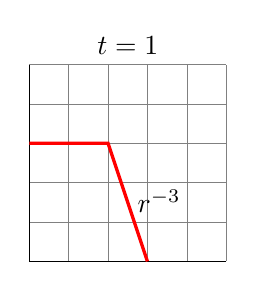
\begin{tikzpicture}
%					Tracé de la grille :
					\draw[step=.5cm,gray,very thin] (0,0) grid (2.5,2.5);
%					Tracé des axes :
					\draw (0,0) -- (0,2.5);
					\draw (0,0) -- (2.5,0);
%					Tracé du graphe :
					\draw[red,very thick] (0,1.5) -- (1,1.5) -- (1.5,0);
%					\draw[red,very thick] (1,1.5) -- (1.5,0);
					\draw (1.25,0.5) node[above right]{$r^{-3}$};
					\draw (1.25,2.5) node[above]{$t = 1$};
				\end{tikzpicture}
			\end{center}
		\end{minipage}\hfill
		\begin{minipage}[b]{0.24\linewidth}
			\begin{center}
				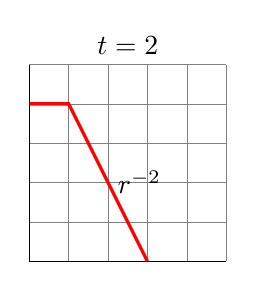
\begin{tikzpicture}
%					Tracé de la grille :
					\draw[step=.5cm,gray,very thin] (0,0) grid (2.5,2.5);
%					Tracé des axes :
					\draw (0,0) -- (0,2.5);
					\draw (0,0) -- (2.5,0);
%					Tracé du graphe :
					\draw[red,very thick] (0,2) -- (0.5,2) -- (1.5,0);
%					\draw[red,very thick] (0.5,2) -- (1.5,0);
					\draw (1,1) node[right]{$r^{-2}$};
					\draw (1.25,2.5) node[above]{$t = 2$};
				\end{tikzpicture}
			\end{center}
		\end{minipage}\hfill
		\begin{minipage}[b]{0.20\linewidth}
			\begin{center}
				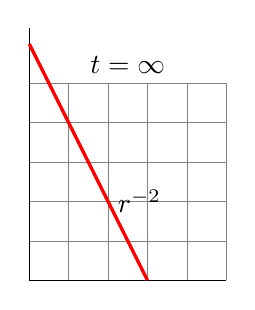
\begin{tikzpicture}
%					Tracé de la grille :
					\draw[step=.5cm,gray,very thin] (0,0) grid (2.5,2.5);
%					Tracé des axes :
					\draw (0,0) -- (0,3.2);
					\draw (0,0) -- (2.5,0);
%					Tracé du graphe :
					\draw[red,very thick] (0,3) -- (1.5,0);
					\draw (1,1) node[right]{$r^{-2}$};
					\draw (1.25,2.5) node[above]{$t = \infty$};
				\end{tikzpicture}
			\end{center}
		\end{minipage}
		\caption{Schéma d'évolution dynamique d'un amas globulaire.\label{schema-effondrement}}
	\end{figure}


%(~la pente $-4$ avec laquelle commence le schéma vient des résultats de simulations numériques~).
%La question à laquelle nous souhaitons répondre est : comment expliquer qu'un amas évolu en augmentant la densité de son cœur et en diminuant la pente avec laquelle le halo décroit ?

%Pour commencer, un amas doit, lorsqu'il est à l'équilibre, suivre un modèle de \textsc{King} ou de sphère isotherme en boîte. Par conséquent, notre amas est au Viriel.
%De plus, le cœur est un systéme auto-gravitant décrit par la thermodynamique. L'un de ses propriétés thermodynamique les plus importante à ce niveau est sa capacité calorifique. En effet :
%Nous cherchons à concentrer la matière dans le cœur de l'amas, et donc y rajouter de la matière à partir du halo (~qui va se diluer~).
%Pour faire diminuer le rayon de l'orbite d'un astre, il faut augmenter sa vitesse~\footnote{rappel : $v^2 = K\left(\frac{2}{r} - \frac{1}{a}\right)$ avec $K = G\left(M+m\right)$
%pour des interactions à deux corps}, et donc sa température. En se rappelant les résultats sur les diagrammes d'énergie de la sphère isotherme, nous nous rendons bien compte que, si la température
%augmente trop, le cœur va passer dans la zone instable, et s'effondrer.

%Le processus pour faire augmenter la température auquel nous nous attèlerons dans la suite est assez simple : l'amas évolue dans le potentiel galactique ; il va en traverser le disque de façon périodique.
%Moments pendant lesquels il va se faire harceler par des forces de marée qui vont lui faire perdre des étoiles. En considérant la description micro canonique, l'énergie est fixé ; or perdre une étoile
%diminue l'énergie potentielle de l'amas. La température va devoir augmenter pour conserver l'énergie totale constante.

%La perte d'étoile apparaît alors comme un processus intéressant pour expliquer l'évolution observée. Les chapitres suivants nous permettront de déterminer, à l'aide de simulation numérique, si la perte
%d'étoile par effet de marée est suffisante pour l'expliquer.








Cette dernière étude nous montre que plus un amas est âgé, plus la pente de son halo est importante.
Dans le chapitre précédent, nous avons relié la pente au paramètre $W_0$ qui, en plus de jouer sur les pentes, joue sur la densité centrale, comme le montre la figure~\ref{King_Modele-test}.
Par ailleurs, des simulations partant d'un nuage homogène nous apprennent que la pente du halo après sa formation vaut $-4$.
Un amas va donc partir d'une structure cœur-halo avec un cœur de taille importante, un halo de pente $-4$ et va tendre, en vieillissant, vers un amas ayant une densité centrale très élevée dont la pente tend vers $-2$.
Puis après un temps infini, l'amas va tendre vers une sphère isotherme.
C'est ce que représente le schéma suivant.


	\begin{figure}[ht!]
		\begin{minipage}[b]{0.20\linewidth}
			\begin{center}
				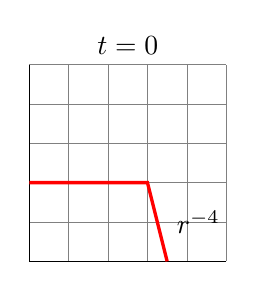
\begin{tikzpicture}
%					Tracé de la grille :
					\draw[step=.5cm,gray,very thin] (0,0) grid (2.5,2.5);
%					Tracé des axes :
					\draw (0,0) -- (0,2.5);
					\draw (0,0) -- (2.5,0);
%					Tracé du graphe :
					\draw[red,very thick] (0,1.0) -- (1.5,1.0) -- (1.75,0);
%					\draw[red,very thick] (1.5,1.0) -- (1.75,0);
					\draw (1.75,0.5) node[right]{$r^{-4}$};
					\draw (1.25,2.5) node[above]{$t = 0$};
				\end{tikzpicture}
			\end{center}
		\end{minipage}\hfill
		\begin{minipage}[b]{0.20\linewidth}
			\begin{center}
				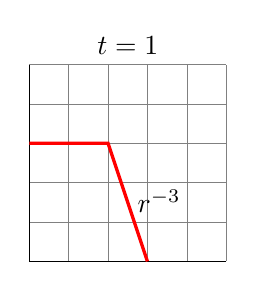
\begin{tikzpicture}
%					Tracé de la grille :
					\draw[step=.5cm,gray,very thin] (0,0) grid (2.5,2.5);
%					Tracé des axes :
					\draw (0,0) -- (0,2.5);
					\draw (0,0) -- (2.5,0);
%					Tracé du graphe :
					\draw[red,very thick] (0,1.5) -- (1,1.5) -- (1.5,0);
%					\draw[red,very thick] (1,1.5) -- (1.5,0);
					\draw (1.25,0.5) node[above right]{$r^{-3}$};
					\draw (1.25,2.5) node[above]{$t = 1$};
				\end{tikzpicture}
			\end{center}
		\end{minipage}\hfill
		\begin{minipage}[b]{0.24\linewidth}
			\begin{center}
				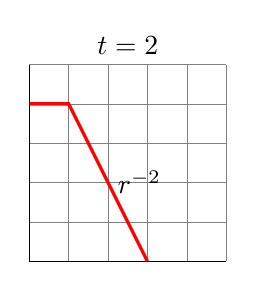
\begin{tikzpicture}
%					Tracé de la grille :
					\draw[step=.5cm,gray,very thin] (0,0) grid (2.5,2.5);
%					Tracé des axes :
					\draw (0,0) -- (0,2.5);
					\draw (0,0) -- (2.5,0);
%					Tracé du graphe :
					\draw[red,very thick] (0,2) -- (0.5,2) -- (1.5,0);
%					\draw[red,very thick] (0.5,2) -- (1.5,0);
					\draw (1,1) node[right]{$r^{-2}$};
					\draw (1.25,2.5) node[above]{$t = 2$};
				\end{tikzpicture}
			\end{center}
		\end{minipage}\hfill
		\begin{minipage}[b]{0.20\linewidth}
			\begin{center}
				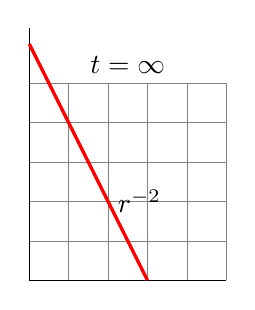
\begin{tikzpicture}
%					Tracé de la grille :
					\draw[step=.5cm,gray,very thin] (0,0) grid (2.5,2.5);
%					Tracé des axes :
					\draw (0,0) -- (0,3.2);
					\draw (0,0) -- (2.5,0);
%					Tracé du graphe :
					\draw[red,very thick] (0,3) -- (1.5,0);
					\draw (1,1) node[right]{$r^{-2}$};
					\draw (1.25,2.5) node[above]{$t = \infty$};
				\end{tikzpicture}
			\end{center}
		\end{minipage}
		\caption{Schéma d'évolution dynamique d'un amas globulaire.\label{schema-effondrement}}
	\end{figure}



Pour expliquer cette évolution, nous devons trouver quels phénomènes, de dynamique gravitationnelle, pourraient diluer le halo et concentrer de la matière au centre de l'amas. Le phénomène qui vient le plus naturellement à l'esprit est la perte d'étoiles, pouvant s'effectuer par 2 scénarios :
\begin{enumerate}
	\item des collisions internes qui éjectent des étoiles de l'amas, permettant ainsi au cœur de s'effondrer en essayant de compenser cette perte d'énergie.
	\item des interactions avec un autre objet massif qui va retirer par effet de marée des étoiles à l'amas, causant l'effondrement de son cœur.
\end{enumerate}
C'est ce deuxième scénario que nous allons tenter d'étudier.
















%Si la température cinétique du halo augmente, celle du
%cœur va changer pour s'adapter. La capacité calorifique à volume
%constant est négative pour le cœur (~et pour tout système
%auto gravitant~) :
%\begin{align*}
%	E_p &= -2E_c & \text{(~Viriel~)} \\
%	\Rightarrow E &= E_p + E_c = -E_c \\
%	\intertext{or}
%	E_c &\varpropto T \Rightarrow E\varpropto -T \\
%	\intertext{donc}
%	\Rightarrow C_v &= \frac{\partial E}{\partial T} < 0
%\end{align*}
%Cela implique que notre système ne peut que prendre de l'énergie.

%Si la température du cœur augmente, la vitesse de rotation des
%étoiles va augmenter (~$E_c\varpropto T\varpropto v$~), et donc
%leur demi grand axe va diminuer~\footnote{rappel : $v^2 =
%K\left(\frac{2}{r} - \frac{1}{a}\right)$ avec $K = G\left(M+m\right)$
%pour des interactions à deux corps}.
%En conséquent la densité au centre du cœur augmente, augmentant
%ainsi le contraste de densité. Si la température augmente
%suffisamment, le contraste de densité du halo va dépasser la
%valeur critique $\R_c^H$ (~l'énergie est fixé, seul la
%température change, nous utilisons donc la description micro
%canonique~). Le cœur va alors devenir instable.


%	L'interprétation semble simple ici : par exemple : quand les étoiles
%	ont des vitesses de rotation élevées la sphère a une température élevée,
%	et donc sa capacité calorifique à volume constant, $C_v = \frac{\partial H}{\partial T} < 0$
%	(~négatif car $E_p=-2E_c\Rightarrow H=E_c+E_p=-E_c\varpropto-T$~),
%	tend vers $0$ : elle ne peut plus acquérir d'énergie.
%	Si on dépasse la limite de température, elle va devoir se \og~réorganiser~\fg pour
%	rester à l'équilibre et donc pour retourner à un contraste de densité $\R < \R^\beta_c$.
%	Le raisonnement est le même pour la limite en énergie.


	\section{Que peut-on dire des autres ...!}
		
